\begin{ex}
   (Puc) Quer-se colorir o mapa da figura, de modo que dois países vizinhos não sejam  pintados com a mesma cor. Qual o número mínimo de cores que se deve usar?
 \begin{center}
     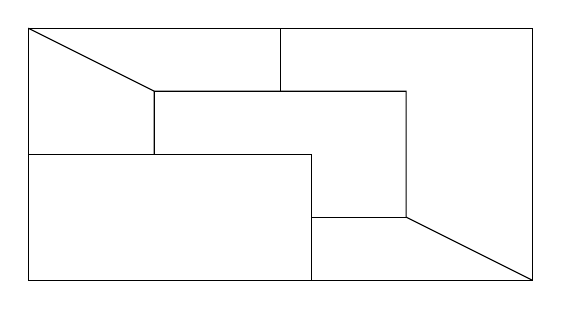
\begin{tikzpicture} [scale = 0.4]
     \draw (0,0) -- (0,8) --(16,8) -- (16,0) -- (0,0);
     \draw (0,4) --(9,4) -- (9,0);
     \draw (4,4) -- (4,6)-- (12,6)-- (12,2)--(16,0);
     \draw (4,6) -- (0,8);
     \draw (9,2) -- (12,2);
     \draw (8,6) -- (8,8);
     \end{tikzpicture}
 \end{center}
    \begin{enumerate}[(a)]
    \item 3
    \item 4
    \item 5
    \item 6
    \item 7
    \end{enumerate}
      \begin{sol}
        resposta: b\\
        4 cores
      \end{sol}
\end{ex}